\documentclass[12pt, a4paper, reprint, nofootinbib, twoside,  showkeys]{revtex4-1}
\usepackage[utf8]{inputenc}
\usepackage[T1]{fontenc}

\usepackage{xcolor}
\usepackage{pgfplots}
\usepackage{subfigure}
\usepackage{graphicx}


\usepackage{lipsum}
\usepackage{mathtools}
\usepackage{physics}
\usepackage{amsfonts}
\usepackage{amssymb}
\usepackage{amsmath}
\usepackage{amsthm}
\usepackage{import}
\usepackage{tikz}
\usepackage{hyperref} 
\hypersetup{
	pdftex,
	colorlinks=true,
	linkcolor=blue,
	citecolor=red,
	filecolor=magenta,
	urlcolor=blue,
	pdftitle={Article},
	pdfauthor={Author},
}

\tolerance=1
\emergencystretch=\maxdimen
\hyphenpenalty=10000
\hbadness=10000
%==================================================================================
\begin{document}
	\title{Parameter Estimation of Coupled Oscillation System through Markov Chain Monte Carlo Method}
	\author{Chang-Mao Yang}
	\email{409220055@alum.ccu.edu.tw}
	\author{Pi-Hui Tuan}
	
	\affiliation{National Chung Cheng University, Department of Physics}
	\date{\today}
%_____________________________________________________________________________________
\begin{abstract}
	An experimental system for oscillators coupled through homemade springs with unknown spring constants was built to explore the parameter optimization issue based on the Markov Chain Monte Carlo (MCMC) method. By using two ultrasonic distance sensors with an Arduino circuit, the real-time displacement data for coupled oscillators were measured and directly monitored on a designed webpage. To estimate the unknown spring constants, the analytical solutions for the time-dependent displacement of coupled oscillators were derived using Lagrange mechanics. These solutions were then used to search for optimal parameters that align with the experimental results. It is confirmed that after assigning a proper distribution function for the fitting errors, the unknown spring constants can be well determined by the Metropolis-Hastings algorithm of the MCMC method with high computation efficiency.
\end{abstract}
	\keywords{Coupled Oscillators, Markov Chain Monte Carlo, Arduino}
	\maketitle
%_____________________________________________________________________________________
\section{Introduction}
	Parameter estimation and optimization plays an important role in data analysis and modeling across various scientific fields. The conventional least square optimization, while straightforward, can become computationally intensive as the dimensionality of parameters increases. The Markov Chain Monte Carlo (MCMC) method, leveraging probability analysis of random variables, offers a more efficient approach to this challenge. MCMC, especially its Metropolis-Hastings variant, has found extensive applications in computational physics, including but not limited to gravitational wave data analysis and quantum field theory simulations.

Coupled oscillators serve as a paradigmatic model, providing insights into solid-state physics phenomena such as lattice vibrations and atomic interactions. In this study, we apply the MCMC method to estimate the parameters of a coupled oscillator system characterized by three unknown spring constants. Our findings suggest that the MCMC method, in comparison to the traditional least square error analysis, not only reduces computational demands but also yields more precise parameter estimations.
%_____________________________________________________________________________________
\section{Analytical Model}
	Our experimental equipment can be interpreted as shown in FIG. (\ref{fig:system}).
	\begin{figure}[h]\centering
	\import{./}{image/figure.tex}
	\caption{Coupled Oscillation system with three springs and two masses.}
	\label{fig:system}
	\end{figure}
	The system's Lagrangian is represented by 
	\begin{equation}
	L = \frac{1}{2}\sum_{i=1}^{2}m_i \frac{d^2x_i}{dt^2}
		-\frac{k_1x_1^2+k_2\left(x_1-x_2\right)^2+k_3x_2^2}{2},
	\end{equation}
	where $m_i$ is the mass of $i^{\rm th}$ oscillator and $\left(k_1,k_2,k_3\right)$ are the spring constants. Using Euler-Lagrange equation, we obtain a set of the second-order differential equations
	\begin{equation}
	\frac{d^2}{dt^2}\begin{pmatrix}x_1\\ x_2\end{pmatrix} =
	\begin{pmatrix}
	\displaystyle - \frac{k_1+k_2}{m_1}	&\displaystyle  \frac{k_2}{m_1}\\
	\displaystyle  \frac{k_2}{m_2} 		&\displaystyle  -\frac{k_2+k_3}{m_2}
	\end{pmatrix}
	\begin{pmatrix}x_1\\ x_2\end{pmatrix}.
	\end{equation}
	After some algebra, the general expressions for the time-dependent displacement $x_1\left(t\right)$ and $x_2\left(t\right)$ can be exactly solved.
%_____________________________________________________________________________________
\section{Experimental Equipment}
	The photograph of the experimental setup is shown as FIG. (\ref{fig:exp-system}).
	\begin{figure}[h]
	\centering
	\includegraphics[width=0.5\textwidth]{image/system_cleanup.jpg}
	\caption{Experimental setup of the Coupled Oscillators system.}
	\label{fig:exp-system}
	\end{figure}
	The setup includes a standard pulley track and two carts with negligible friction for general physics experiment. Three homemade springs made by white iron wire with unknown spring constants were used to connect the two carts and the end stands to form a coupled oscillator system. Two ultrasonic distance sensors were housed in the 3D-printing frames at the end stands as well as connected to the central Arduino circuit board to record the motion of the two oscillators respectively. Additionally, a customized webpage on a GitHub repository was designed for accessing and visualizing the measured displacement data by the sensors in real time. 
	Through this setup,  the time series $\left\{t_j\right\}$ and the corresponding position series $\left\{x_{1,j}\right\}$ and $\left\{x_{2,j}\right\}$ for the $j^{\rm th}$ step for data acquisition can be measured and recorded to characterize the dynamics of coupled oscillators. 

%_____________________________________________________________________________________
\section{Desired Distribution}
Theoretically, once the system parameters (such as the oscillator masses $\left(m_1,m_2\right)$, the spring constants $\left(k_1,k_2,k_3\right)$, and the initial conditions) are given, $x_1\left(t\right)$ and $x_2\left(t\right)$ of the coupled oscillators is determined. Therefore, once the masses and the initial released positions for the two oscillators have been measured beforehand, the acquired real-time data of $\left\{t_j\right\}$, $\left\{x_{1,j}\right\}$ and $\left\{x_{2,j}\right\}$ can provide the boundary conditions for estimating the unknown $\left(k_1,k_2,k_3\right)$ 
by optimally fitting the numerical calculation to the experimental data. We define the fitting error as
\begin{equation}
\mathrm{err}\left(k_1,k_2,k_3\right) = \sum_{i=1}^{2}\sum_{j=0}^{N-1}\frac{\left(x_i\left(t_j\right) - x_{i,j}\right)^2}{N},
\end{equation}
where $N$ is the total time steps for the acquired data.

To find the values of $ k_1 $, $ k_2 $, and $ k_3 $ that correspond to the minimum error, we define the desired distribution as
\begin{equation}
p\left(k_1,k_2,k_3\right) = \exp\left(-\text{err}\left(k_1,k_2,k_3\right)\right), \quad \text{with }\mathrm{err}\in [0,\infty),
\end{equation}
In other words, the optimized values for $\left(k_1,k_2,k_3\right)$ correspond to the maximum of the distribution function. In practice, the distribution $p$ may have many local maxima degrading the accuracy for the optimization strategy. To solve this problem, we used the concept of Gamma correction commonly adopted in image processing to improve the contrast between the peak and valley values for the distribution. The distribution with improved contrast can be given by
\begin{equation}
P = p^{\gamma},\quad p\in (0,1],
\end{equation}
The FIG. (\ref{fig:gamma-plot}) shows the relations between $p$ and $P$ under different.
\begin{figure}[h]

	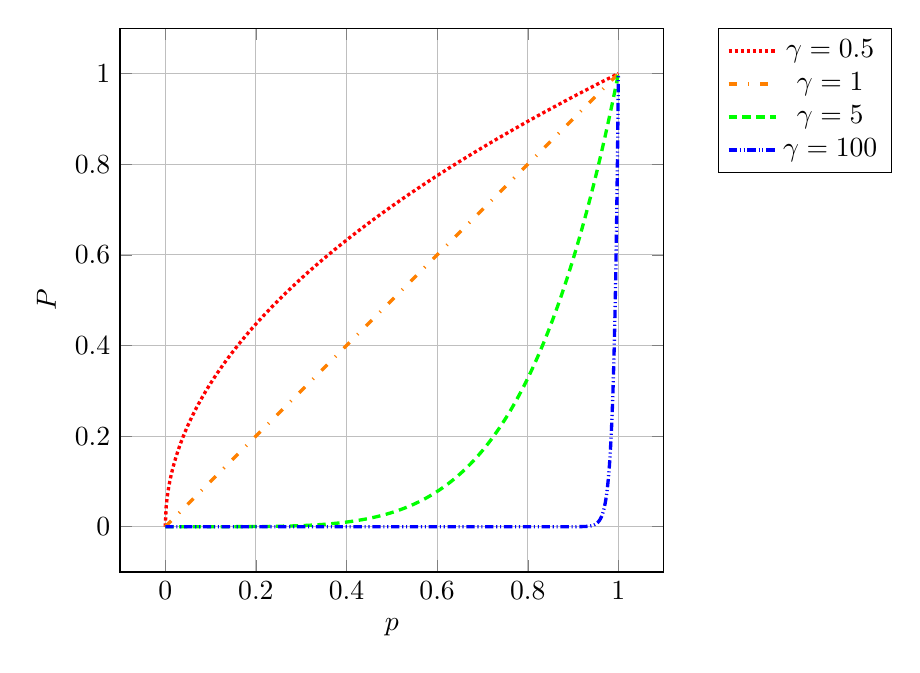
\begin{tikzpicture}
		\begin{axis}[
			xlabel={$p$},ylabel={$P$},grid=both,
			width=0.7\linewidth,height=0.7\linewidth,
			legend style={at={(1.1, 1.0)},anchor=north west}
		]
		\addplot [red, densely dotted, domain=0:1, samples=500, line width=1.2pt] {x^(0.5)};
		\addlegendentry{$\gamma=0.5$}
		
		\addplot [orange, loosely dashdotted, domain=0:1, samples=500, line width=1.2pt] {x};
		\addlegendentry{$\gamma=1$}
		
		\addplot [green, densely dashed, domain=0:1, samples=500, line width=1.2pt] {x^(5)};
		\addlegendentry{$\gamma=5$}
		
		\addplot [blue, densely dashdotdotted, domain=0:1, samples=500, line width=1.2pt] {x^(100)};
		\addlegendentry{$\gamma=100$}
		
		\end{axis}
	\end{tikzpicture}
	\caption{Plot $P=p^\gamma$ for some $\gamma$ values, where $x\in[0,1]$.}
	\label{fig:gamma-plot}
\end{figure}

%_____________________________________________________________________________________
\section{Markov Chain Monte Carlo and Result}
With the defined distribution function $P$, we then perform the MCMC simulation based on the Metropolis-Hastings algorithm to resolve the parameter space of $\left(k_1,k_2,k_3\right)$. By sampling 100,000 different combinations of three spring constants, we were able to obtain the simulated posterior distribution. The FIG. (\ref{fig:MCMC_corner}) illustrates one of the simulation results which provides the behavior of distribution function under various combinations of the $\left(k_1,k_2,k_3\right)$ space. From the subplots on the main diagonal of FIG. (\ref{fig:MCMC_corner}), the statistical distributions corresponding to spring constants $k_1$, $k_2$ and $k_3$ are clearly presented. Although showing slightly skewed trends, the statistical distributions still nicely resemble normal distributions, which ensures accurate estimations for the three unknown spring constants as shown by the intersections of the red lines in FIG. (\ref{fig:MCMC_corner}). 
\begin{figure}[h]
\centering
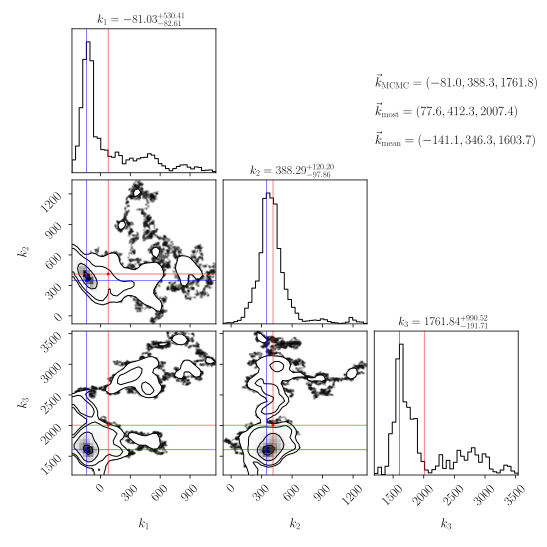
\includegraphics[width=\linewidth]{image/MCMC_corner.pdf}
\caption{Posterior distributions of the spring constants $k_1$, $k_2$, and $k_3$ using the corner package. The plots on the main diagonal represent the one-dimensional distributions of each parameter, while the plots in the lower triangle show the two-dimensional distributions between pairs of parameters. The red lines mark the median positions, corresponding to values of $101.03\,(\mathrm{N/m})$, $175.97\,(\mathrm{N/m})$, and $265.02\,(\mathrm{N/m})$ for $k_1$, $k_2$, and $k_3$, respectively, in this figure.}
\label{fig:MCMC_corner}
\end{figure}

Considering the precision of the experiment, the spring constants are analyzed with two significant figures for the decimal values. The FIG. (\ref{fig:position_compare}) shows the comparison between the experimental measurements for $\left\{x_{1,j}\right\}$ and $\left\{x_{2,j}\right\}$ and the numerical calculation of $x_1\left(t_j\right)$ and $x_2\left(t_j\right)$ based on the parameters estimated by the MCMC method. Although with some minor errors from experimental imperfections, it can be clearly seen that the numerical simulation well describes the dynamical trends for the experimental coupled oscillators. It is believed that this work can provide a pedagogically beneficial demonstration for using the MCMC method to perform efficient parameter estimation for the classic model in physics.
\begin{figure}[h]
\centering
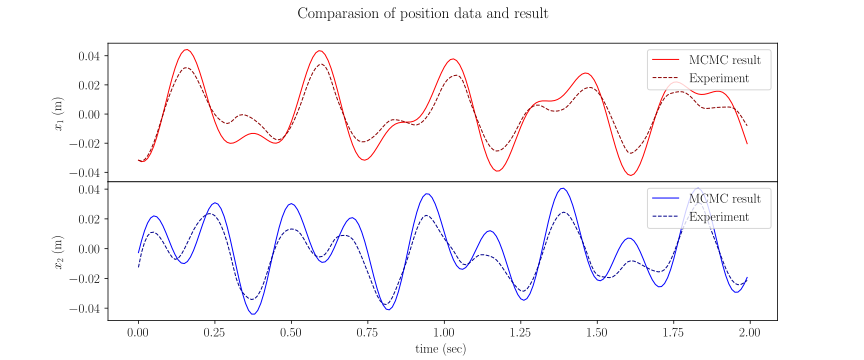
\includegraphics[width=\linewidth]{image/position_compare.pdf}
\caption{Comparison of the MCMC result (solid line) with the experimental data (dashed line).}
\label{fig:position_compare}
\end{figure}

\section{Conclusion}
In this study, we successfully applied the Markov Chain Monte Carlo (MCMC) method, specifically the Metropolis-Hastings algorithm, to analyze the coupled oscillators system. By defining the desired distribution and employing the MCMC method, we were able to explore the parameter space of the spring constants $k_1$, $k_2$, and $k_3$, obtaining a simulated posterior distribution that closely resembles a normal distribution.

Despite minor irregularities and errors in the experimental data, possibly attributed to the experimental equipment, the comparison between the MCMC result and the experimental data demonstrated a good fit. The use of the corner package allowed for detailed visualization of the posterior distributions, with the median positions providing valuable insights into the system's behavior.

The findings of this study not only enhance our understanding of the coupled oscillators model but also showcase the efficacy of the MCMC method in overcoming the limitations of traditional minimization techniques. The approach presented here can be extended to other complex physical systems, offering a robust and efficient tool for parameter estimation and system analysis.

Future work will focus on improving the experimental setup to reduce potential errors and conducting more data collection. Additionally, we plan to compare the simulation results with springs of different elastic constants and even explore the system's dynamics further by altering the dimensionality of the parameter space through the addition of more elastic constants. These efforts will contribute to a deeper understanding of the behavior of coupled oscillators and the development of more precise models and analytical methods.


	



	
	
	\begin{thebibliography}{4}
		\bibitem{Schwartz}  M. "Schwartz, Lecture 3: Coupled oscillators", URL: \url{https://scholar.harvard.edu/files/schwartz/files/lecture3-coupled-oscillators.pdf}
		\bibitem{Hastings} W.K. Hastings, "Monte Carlo sampling methods using Markov chains and their applications," Biometrika, vol. 57, no. 1, pp. 97–109, 1970.

		
		
		%https://arxiv.org/abs/1912.10997
	\end{thebibliography}
	
\end{document}




